%PLS and pollen pie maps
\begin{figure}
\centering
\begin{tabular}{c}
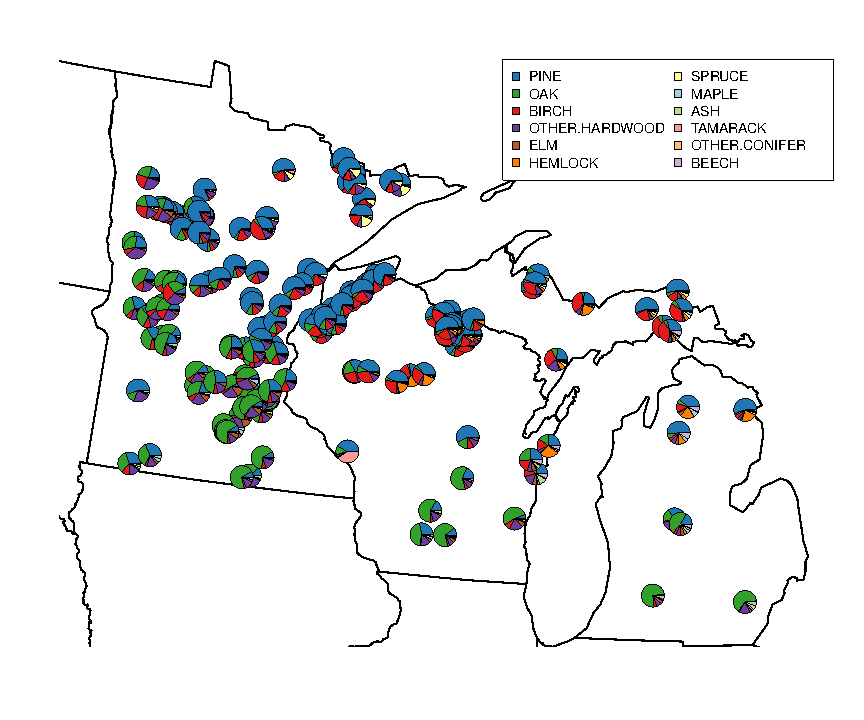
\includegraphics[width=5in]{figures/pie_plot_pollen_ALL_v0_3.png} \\
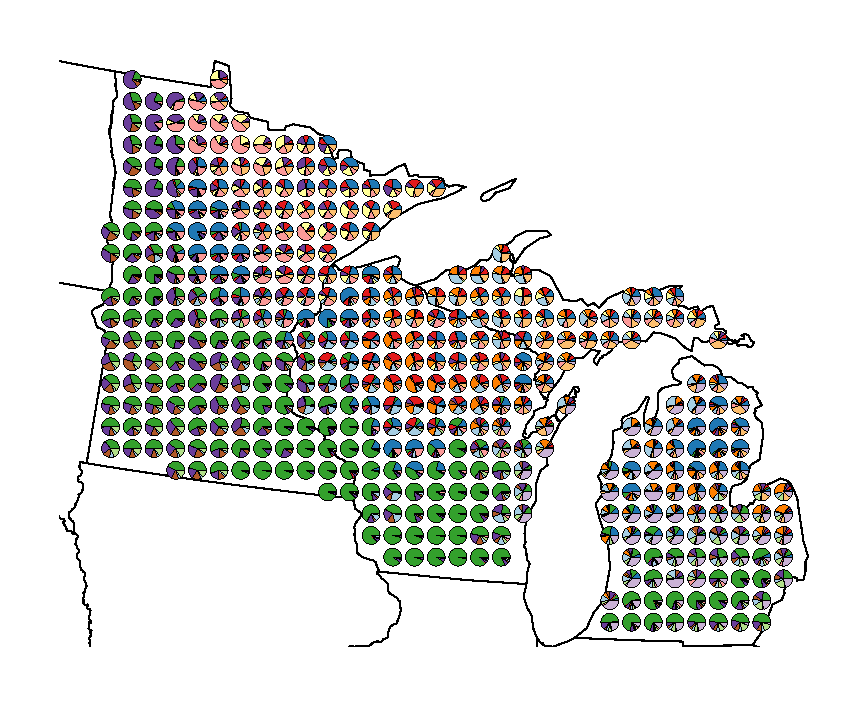
\includegraphics[width=5in]{figures/pie_plot_pls_ALL_v0_3.png}
\end{tabular}
\caption[Pie maps]{\internallinenumbers \doublespacing Pie maps depicting the relative composition of tree genera of
  pollen (top) and PLS vegetation (bottom) from the data. Note that
  the PLS data has been aggregated from 8 km to 32 km resolution for
  illustrative purposes.}
\label{fig:pie}
\end{figure}

%potential pollen maps by taxon
\begin{figure}
\centering
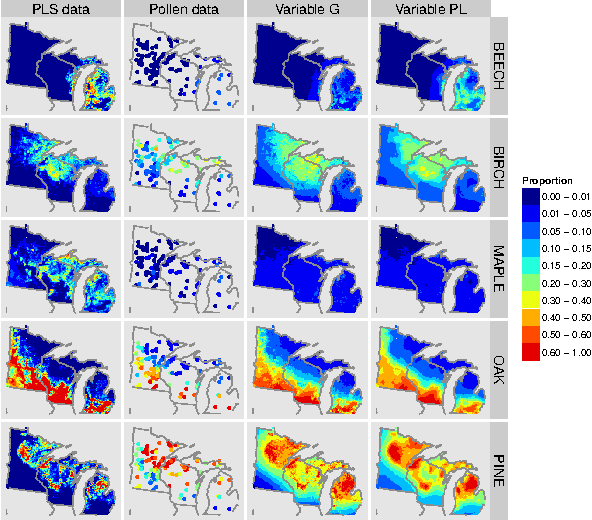
\includegraphics[width=7in]{figures/map_pls_pollen.png}
\caption[PLS data, pollen data, predicted pollen heat
  maps]{\internallinenumbers \doublespacing Heat maps of the PLS data, pollen data, and
  predicted sediment pollen for the variable Gaussian (GK) and
  power-law (PLK) kernel models for a subset of modelled taxa.}
\label{fig:maps_pp}
\end{figure}

%pollen raw versus scaled focal
\begin{figure}
\centering
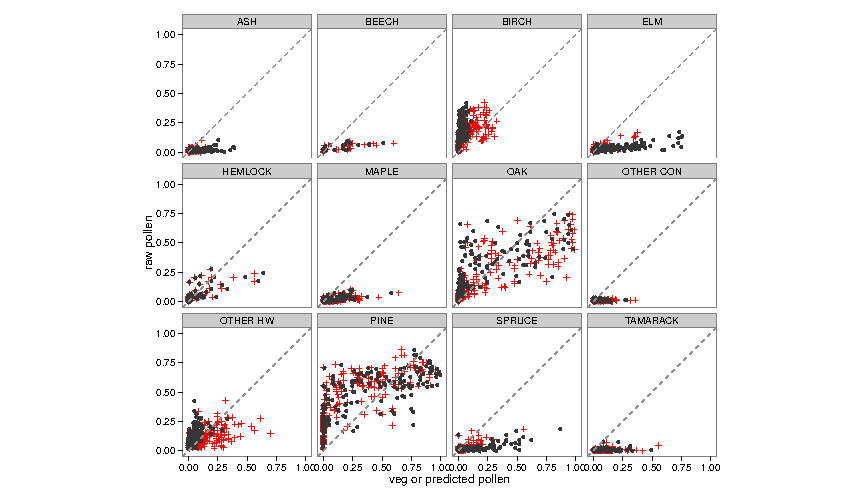
\includegraphics[width=7in]{figures/pollen_phi_scaled_pl_Ka_Kgamma.png}
\caption[Pollen-vegetation scatter, $\phi$-scaled]{\internallinenumbers \doublespacing
  Pollen proportions plotted against local vegetation proportions (red
  crosses) or local vegetation proportion scaled by the pollen
  production factor $\phi_k$ for the variable power-law kernel (PLK)
  model (black dots).}
\label{fig:focal_scaled}
\end{figure}

%pollen raw versus predicted
\begin{figure}
\centering
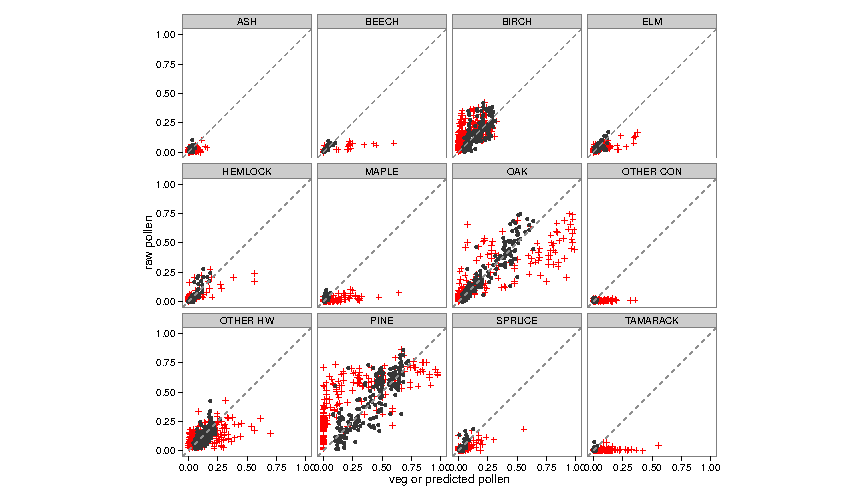
\includegraphics[width=7in]{figures/pollen_preds_pl_Ka_Kgamma.png}
\caption[Pollen-vegetation scatter, predicted]{\internallinenumbers \doublespacing Pollen
  proportions plotted against local vegetation proportions (red
  crosses) or model-predicted pollen for the variable power-law kernel
  (PLK) model (black dots).}
\label{fig:preds}
\end{figure}

%phi (differential production)
\begin{figure}
\centering
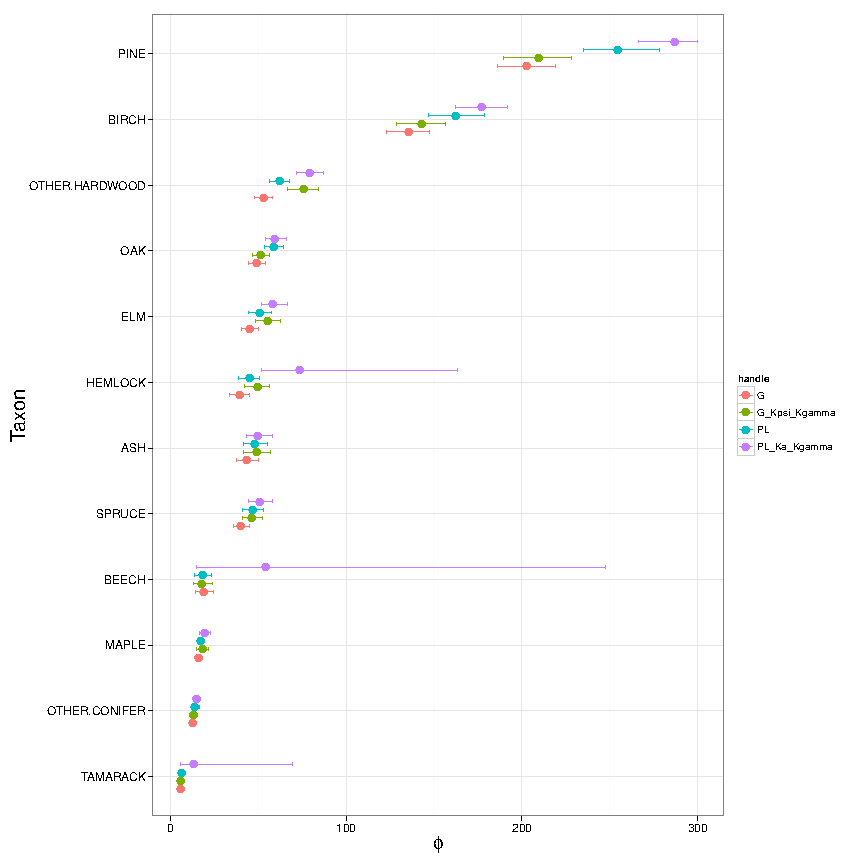
\includegraphics[width=7in]{figures/phi.png}
\caption[]{\internallinenumbers \doublespacing Mean values and 95\% credible intervals for differential
  production parameter $\phi$, by taxon for the four considered
  models  (GK and PLK base and variable).}
\label{fig:phi}
\end{figure}

%proportion pollen versus radius
\begin{figure}
\centering
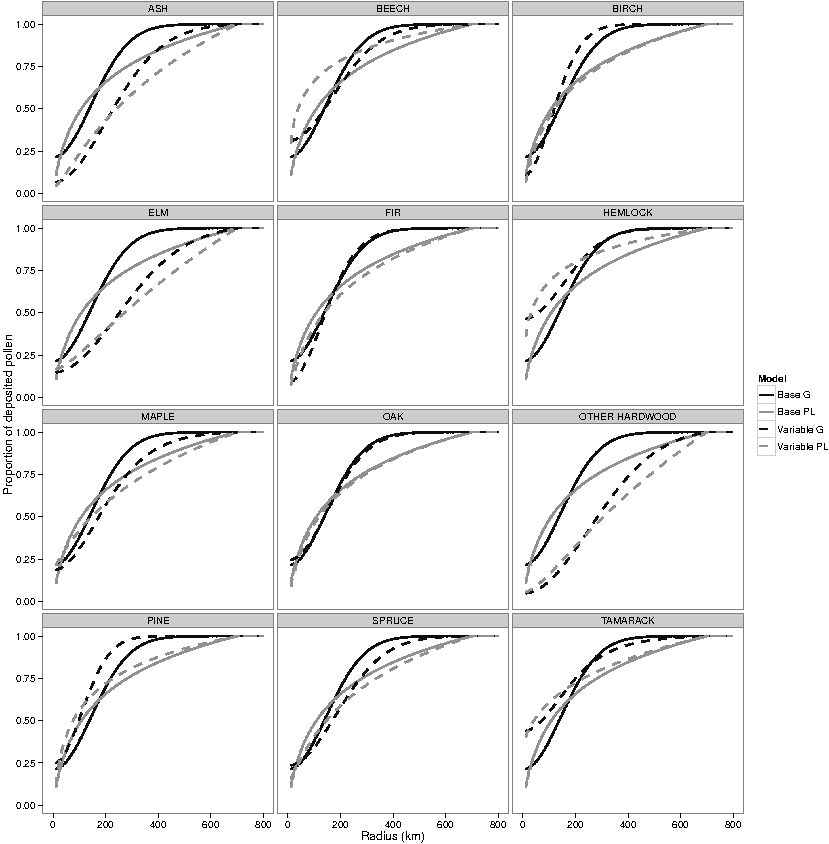
\includegraphics[width=7in]{figures/kernel_discrete_cdfs.png}
\caption[]{\internallinenumbers \doublespacing The proportion of deposited (or accumulated) pollen plotted
  as a function of radius for each of the modelled taxa and for each
  of the four considered models (GK and PLK base and variable).}
\label{fig:cdf}
\end{figure}


%PPE scatter
\begin{figure}
\centering
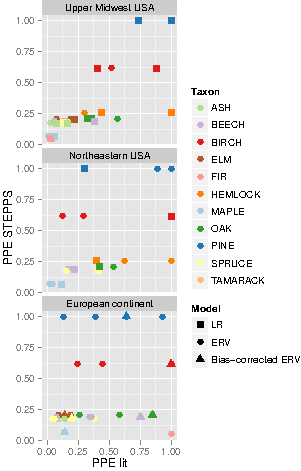
\includegraphics[width=4in]{figures/PPEs_panels.png}
\caption[]{\internallinenumbers \doublespacing Pollen productivity estimates (PPEs) from STEPPS versus sets
  of previously published PPEs from different geographical regions
  (Upper Midwest USA, Northeastern USA, European continent). Published
  PPE data sets were generated using linear regression (LR), extended
  R-value (ERV), or bias-corrected ERV models.}
\label{fig:ppe}
\end{figure}

%SV scatter
\begin{figure}
\centering
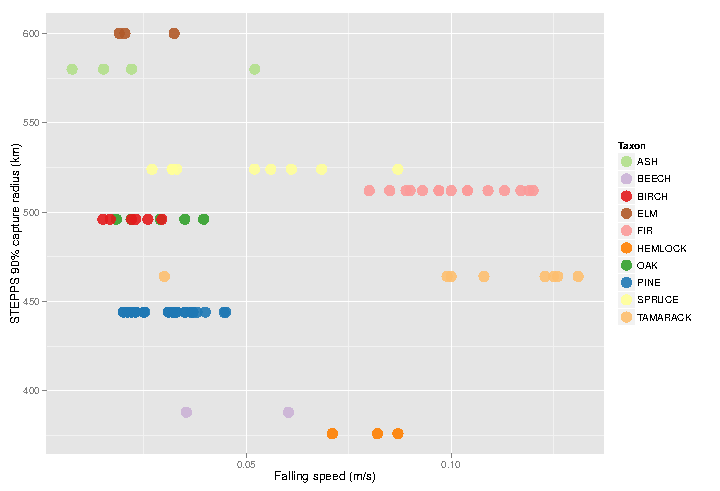
\includegraphics[width=7in]{figures/SVs_90_single.png}
\caption[]{\internallinenumbers \doublespacing Scatter plot of the STEPPS 90\% capture radius versus
  measured falling speeds.}
\label{fig:svs}
\end{figure}

%PLS estimates, STEPPS estimates, and uncertainty for the best model
\begin{figure}
\centering
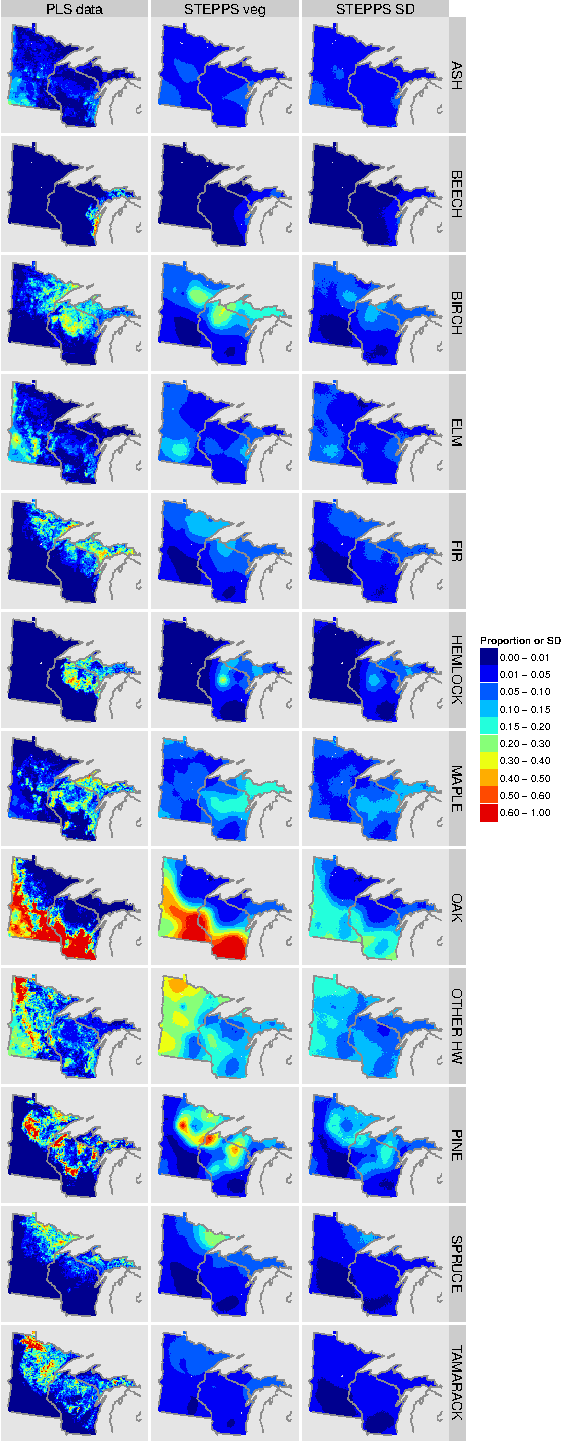
\includegraphics[width=3.2in]{figures/maps_PLS_STEPPS_SD.png}
\caption[]{\internallinenumbers \doublespacing Heat maps of the PLS data, STEPPS
  composition estimates and the standard deviation of the posterior
  sample, based on the variable PLK model.}
\label{fig:maps_pls_stepps_sd}
\end{figure}




